\documentclass[sigconf, 6pt]{acmart}

\usepackage{graphicx}
\usepackage{stfloats}
\usepackage{titlesec}

\titleformat{\section}
  {\normalfont\fontsize{9}{9}\bfseries}{\thesection}{1em}{}


\settopmatter{printacmref=false} % Removes citation information below abstract
\renewcommand\footnotetextcopyrightpermission[1]{} % removes footnote with conference information in first column
\pagestyle{plain} % removes running headers

\title{\textbf{Comparing Optimization Algorithms on the Ellipsoid}}
\author{Ravinder Rai}
\date{\today}


\begin{document} 


\begin{abstract}
In this report, we look at a few different types of optimization algorithms, one being the quasi-newton algorithm, and the other two being variants of the evolution strategy algorithm. All algorithms seek to solve the problem of finding a minimum value of a given test problem, which in this case is a convex quadratic test problem. We compare these algorithms by essentially comparing the number of function evaluations used to find the minimum value of the test problem. The results are collected by varying a certain parameter one at a time. The algorithm of most interest is one of the Evolution Strategy algorithms, and as such is analysed in all results. The first result compares the two Evolution Strategy algorithms, clearly displaying which one is better. The second result then also considers the quasi-newton algorithm, with a separable and non-separable test problem.
\end{abstract}
\maketitle

\section{Introduction}
\label{sec:intro}

In this paper, we compare the cost of three optimization algorithms to find the minimum value of a certain test problem, that being an ellipsoid. The first algorithm is a quasi-newton algorithm, and is implemented by using a Matlab function, fminunc. The second and third algorithms are evolution strategy algorithms, called the $(1+1)$-ES algorithm and the covariance matrix adaptation algorithm ($(u/u,\lambda)$-CMAES). To complete experiments, we vary certain parameters and observe how the changes affect the cost as it relates to the number of function evaluations (fcount for short). One result of this report shows that $(u/u,\lambda)$-CMAES is a better algorithm for the ellipsoid than $(1+1)$-ES. The next and more interesting result compares the $(u/u,\lambda)$-CMAES and fminunc algorithms on both the separable and non-separable ellipsoid, where non-separable essentially means rotated. The rotation is of interest because the CMAES algorithm is designed to handle this kind of ill-conditioning (i.e. unaligned axis), and so we expect it to do better than the fminunc algorithm.


\section{Preliminaries}
\label{sec:pre}
Here we highlight some important tools used in this paper. The first tool is the fminunc function in Matlab, which tries to minimize a given test problem. The fminunc function will follow the quasi-newton algorithm here, and works by starting with some initial $x_0$ value, and making steps in an optimal direction to find a local minimum, by approximating the Hessian matrix. The Hessian matrix approximation is updated as the algorithm iterates, and the update variant we consider here is the bfgs version. Now, note that the $(1+1)$-ES algorithm differs from fminunc, in that it does not use a Hessian, and simply checks/compares function values at every iteration, following some update until a target value is reached. The $(u/u,\lambda)$-CMAES differs even further, as it checks function values of many initial values and takes averages every iteration. Also, it adapts its step size every iteration via a covariance matrix to allow for faster convergence. The test problem here, the ellipsoid, is of the form: $f(x)=\sum^n_{i=1}\alpha^{(i-1)/(n-1)} x_i^2$. To make the ellipsoid non-separable, we rotate it via an orthogonal matrix, $O$. Note, the idea for this was burrowed from \cite{orthogonal}.


\section{Algorithms}
\label{algorithm}
The quasi-newton algorithm, given by the fminunc function in Matlab, works as follows. We first start with an initial starting point, $x_0$ (given by the randn function in Matlab). Then we set our stopping criteria options for Matlab's fminunc function, of which we only care about the target function value and stopeval, so all others are set to be either arbitrarly small or large to ensure that fminunc does not stop for any of these reasons. This function will take inputs: $n$ for the dimension, the constant $\alpha$, a target function value, the stopeval, an orthogonal matrix $O$, and the Hessian update, and returns the variables that we recorded. Note, some of the code to implement this was borrowed from \cite{MathWorks}. The next algorithm is the $(1+1)$-ES algorithm, and works a bit differently. First pick an initial (parent) point, $x_0$, and then $\gamma$, and then define $y = x + z*\gamma$ (offspring), where $z$ is a vector with random elements, and gamma is some update variable (initially $1$). Then simply check function values at $y$ and $x$ to get the next $x$ value, and update $\gamma$ by the $1/5$ rule. Next is the $(\mu / \mu, \lambda)$-CMAES algorithm, which works similarly but with two main differences. The first difference is that there are $\mu$ parents and $\lambda$ offspring, and averages are taken to get function values over $\mu$ chosen values. The second difference is that $y = x + z*A*\gamma$ instead, where $A$ is the covariance matrix, meant to adapt step size to allow for faster convergence. The code for this was taken and modified from \cite{pureCMAES}.

Finally, using these functions, we can iterate through chosen values of $\alpha$ while holding $n$ constant to display plots of the fcount against these varying parameters. In the plots below, we consider the SP1, which is the average of the number of function evaluations of successful runs divided by the ratio of successful runs. The idea of using SP1 comes from \cite{derivativefree}, and is meant to estimate the fcount of an algorithm as if it were restarted unitl it successfully reached the target function value. Also, these algorithms are used to reproduce the ellipsoid plots in Figure 1 in \cite{derivativefree}, but with slightly different parameters. 



\section{Results and Discussion}
\label{result}


\begin{figure}[h]
\centering
  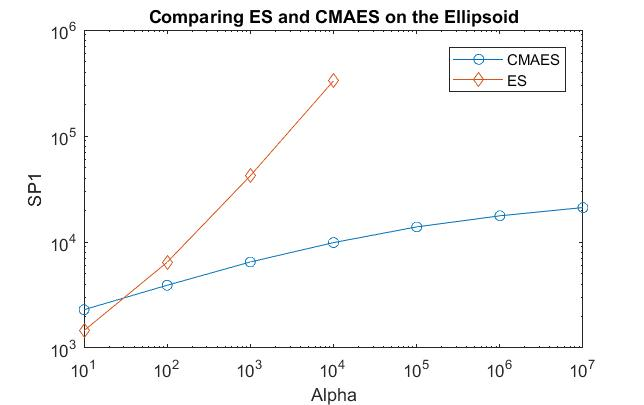
\includegraphics[height = 5cm, width=9cm]{A3ESstrategies.jpg}
  \caption{This loglog plot displays SP1 (taken over 5 runs) against $\alpha$, while $n=20$. Target is $1e-6$, and the stopeval is $10^6$.}
  \label{fig:ES}
\end{figure}

The first result is shown in Figure \ref{fig:ES} and shows the difference in performance of the ES algorithm compared to the CMAES algorithm. In this case, we kept $n=20$ constant, as we are not interested in varying the dimension here. It seems clear that the CMAES algorithm is better for all but smaller values of $\alpha$, and once $\alpha>10^4$, the ES algorithm fails due to the fcount going past the stopeval. This is as expected, as the CMAES algorithm is meant to better handle problems like cigar and ellipsoid functions since they are not as well-conditioned as the sphere.

\begin{figure}[h]
\centering
  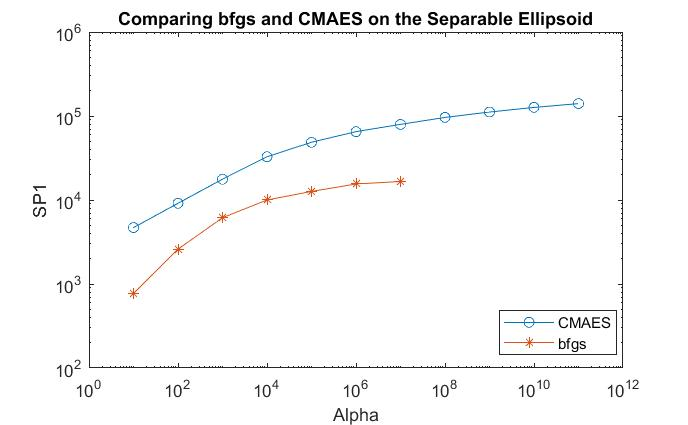
\includegraphics[height = 5cm, width=9cm]{A3separable40.jpg}
  \caption{This plot displays SP1 (taken over 5 runs) against $\alpha$ on the separable ellipsoid, with $n = 40$. Target is $1e-6$, and the stopeval is $10^7$}
  \label{fig:sep}
\end{figure}

Next, since we know that the CMAES algorithm is better than the ES algorithm, we leave it out of the remaining plots, and so Figure \ref{fig:sep} shows a similar result but with the bfgs algorithm instead. The results in this plot are more interesting, because you can see that as the value of $\alpha$ increases, the bfgs algorithm is clearly better than the CMAES algorithm. However, once $\alpha>10^7$, the bfgs algorithm fails completely (due to numerical errors), and so CMAES is now the better algorithm. Finally, Figure \ref{fig:nonsep} then compares CMAES and bfgs again, but this time with the ellipsoid being rotated by an orthogonal matrix $O$. Since this causes the ellipsoid test problem to become a non-separable test problem, we expect CMAES to outperform bfgs even more than in Figure \ref{fig:sep}. And indeed we see this in that the bfgs algorithm fails for even smaller values of $\alpha$ (again due to numerical errors), this time when $\alpha>10^6$. 

Now, both  Figures \ref{fig:sep} and \ref{fig:nonsep} are attempts at getting similar results as with Figure $1$ from \cite{derivativefree}, and so we compare them here by first noting some parameter changes: $n=40$ instead of $n=20$, the target function value is $1e-6$, instead of $1e-9$, and number of runs is $5$, not $21$. In the separable case for \cite{derivativefree}, success was encountered in every iteration of $\alpha$ for the bfgs algorithm, unlike here. This is probably because they extended the number of runs to $1001$ runs if no success was encountered (for bfgs). Aside from this, both the bfgs and CMAES plots are quite similar to their counterparts in \cite{derivativefree}. In the non-separable case, for the bfgs plot we actually see that it fails after $\alpha>10^7$ in Figure $1$ in \cite{derivativefree}, as compared to $10^6$ here, which makes sense since the dimension is doubled, numerical accuracy issues are likely going to occur earlier. However, in Figure $1$ in \cite{derivativefree} the bfgs plot actually has a larger SP1 value than CMAES at $\alpha = 10^7$. This may be due to bfgs failing a lot, so the fcount gets divided by a small number (success ratio of fminunc reaching the target), thus increasing the value. In terms of the CMAES plots, they seem to be similar, although with higher SP1 values due to a doubled dimension (similarly for bfgs). Thus overall the plots here are pretty similar to the results in \cite{derivativefree}, despite the doubled dimension.

\begin{figure}[h]
\centering
  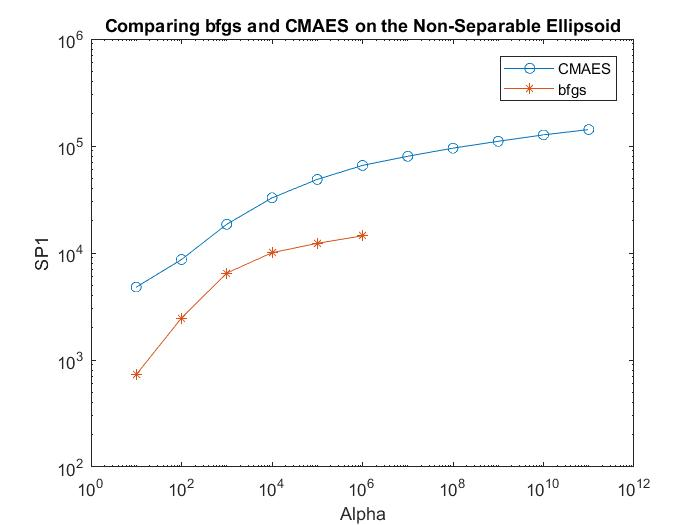
\includegraphics[height = 5cm, width=9cm]{A3nonseparable40.jpg}
  \caption{This plot displays SP1 (taken over 5 runs) against $\alpha$ on the non-separable ellipsoid, with $n = 40$. Target is $1e-6$, and the stopeval allowed is $10^7$}
  \label{fig:nonsep}
\end{figure}

\section{Conclusion}
\label{con}
From the results observed in Figure \ref{fig:ES}, the $(1+1)$-ES algorithm clearly has a higher cost than the CMAES algorithm, which is the expected result since CMAES is designed to better handle test problems like ellipsoids. Another experiment that might be of interest would be to try simpler test problems like the sphere to see if results do not improve much when using the CMAES algorithm since the ES algorithm should handle a sphere well. The results from Figures \ref{fig:sep} and \ref{fig:nonsep} show that the bfgs algorithm is better then the CMAES algorithm, but not for larger values of $\alpha$, and it is even worse when the ellipsoid is rotated. This means that the CMAES algorithm is better when dealing with ill-conditioning and larger values of $\alpha$. Also, since $n$ was doubled here, we showed that bfgs fails for even smaller values of $\alpha$ then in \cite{derivativefree}. Moreover, even though the target value here was different by a factor of $10^3$ and the SP1 was taken over a much smaller number of runs as compared to Figure $1$ in \cite{derivativefree}, these results are fairly similar, and so as a final note, it might be interesting to continue exploring by considering different target and stopeval values.


\bibliographystyle{unsrt}
\addcontentsline{toc}{section}{Bibliography}
\bibliography{A3}


\end{document}